В этой главе собраны разрозненные базовые знания о типах, необходимые для дальнейшего погружения.

\subsection{Алгебраическое представление типа}

% todo algebraic data types are relations between data https://stanford-cs242.github.io/f18/lectures/02-2-algebraic-data-types.html
% todo https://codewords.recurse.com/issues/three/algebra-and-calculus-of-algebraic-data-types

\begin{figure}[h!]
    \centering
    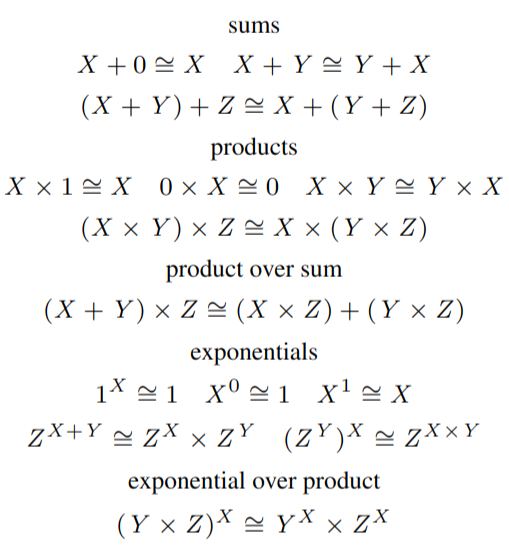
\includegraphics[width=0.4\textwidth]{figs/school-alg}
    \caption{Законы школьной алгебры ностальгии ради~\cite{hinze2010reason}.}
    \label{fig:school-alg}
\end{figure}

% todo isomorphismы и кардинальности
% todo reason isomorphically
% todo connection with cardinalities

\cite[глава 1]{maguire-types}

% todo каноническое представление типа

TODO % todo

\subsection{Представление структур как неподвижной точки функтора}

TODO % todo

\subsection{Полярности и вариантность}

В этом параграфе мы будем рассматривать тему с точки зрения программирования~\cite[глава 3]{maguire-types}, не отдавая должного теории категорий.
Восполнить пробел можно с помощью замечательной статьи, написанной в жанре пьесы~\cite{hinze2012functional}.

\vocab{Ковариантный функтор} --- пара из типового конструктора \texttt{F} и операции на функциях \texttt{fmap :: (a -> b) -> (F a -> F b)}.
Плюс законы о том, что \texttt{fmap} уважает \texttt{id} и композицию.

\begin{minted}{haskell}
    class Functor f where
      fmap :: (a -> b) -> (f a -> f b)
\end{minted}

\begin{figure}[H]
    \centering
    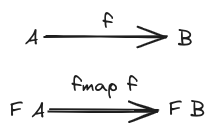
\includegraphics[width=0.3\textwidth]{figs/functor}
\end{figure}

\vocab{Контравариантный функтор} --- пара из типового конструктора и операции на функциях, разворачивающей стрелку.
Плюс соответствующие законы.

\begin{minted}{haskell}
    class Contravariant f where
      contramap :: (a -> b) -> (f b -> f a)
\end{minted}

\begin{figure}[H]
    \centering
    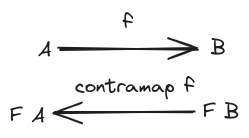
\includegraphics[width=0.3\textwidth]{figs/contra-functor}
\end{figure}

Типовой конструктор можно объявить ковариантным или контравариантным функтором (или никаким из них) относительно типового параметра в зависимости от вида декларации соответствующих конструкторов данных.
А именно, от \vocab{полярности}\footnote{\url{https://existentialtype.wordpress.com/2012/08/25/polarity-in-type-theory/}}\footnote{\url{https://ncatlab.org/nlab/show/polarity+in+type+theory}} позиций, в которых входит этот типовой параметр в декларации.

Попробуем развить интуитивное понимание полярностей.
Рассмотрим некоторое вычисление типа \texttt{F a}.
Параметр \texttt{a} входит в положительной позиции, если все его значения можно извлечь из \texttt{F a}, как в следующих примерах (для извлечения могут понадобиться паттерн-матчинг и аппликация):
\begin{minted}{haskell}
    data F a = L a | R a
    data F a = D a (Int -> a)
\end{minted}

Вхождения, наоборот, отрицательные, если значения соответствующего типа нельзя получить из вычисления, но нужно ему предоставить.
Например, в качестве параметров функций:
\begin{minted}{haskell}
    data F a = F (a -> Int)
    data F a = L (a -> ()) | R Int
\end{minted}
Действительно, для первого примера можно объявить инстанс \mintinline{haskell}|Contravariant|:
\begin{minted}{haskell}
    instance Contravariant F where
      contramap :: (a -> b) -> (F b -> F a)
      contramap g (F f) = F (f . g)
\end{minted}

Можно предположить, что на плюс и минус действуют обычные мультипликативные законы.
И это действительно так.
\begin{itemize}
    \item Плюс на плюс даёт плюс:
    \begin{minted}{haskell}
        data F a = F (Int -> (Int -> a))
    \end{minted}
    \item Плюс на минус (и наоборот) --- минус:
    \begin{minted}{haskell}
        data F a = F ((Int -> a) -> Int)
    \end{minted}
    \item Минус на минус --- плюс, поскольку параметр принимаемой функции выдаётся реализацией вызывающей стороне:
    \begin{minted}{haskell}
        data F a = F ((a -> Int) -> Int)
    \end{minted}
\end{itemize}

Тип от двух положительных параметров можно объявить \vocab{бифунктором}:
\begin{minted}{haskell}
    class Bifunctor f where
      bimap :: (a -> c) -> (b -> d) -> f a b -> f c d
\end{minted}

Тип от двух параметров, положительного и отрицательного, --- \vocab{профунктором}:
\begin{minted}{haskell}
    class Profunctor p where
      dimap :: (c -> a) -> (b -> d) -> p a b -> p c d
\end{minted}

Профункторы являются некоторыми обобщениями функциональной стрелки.
Например, если у нас есть SQL запрос, который по данным возвращает результат, его можно объявить профунктором с семантикой --- добавить пред-обработку входных данных и пост-обработку выходных:
\begin{minted}{haskell}
    dimap serialize deserialize (query :: Sql Text Text) :: Sql Age [User]
\end{minted}

Также понятие вариантности часто встречается в объектно ориентированных языках для обозначения возможности дополнить отношение подтипизации на полиморфные типы (да и вообще в теории подтипизации).

Действительно, \vocab{отношение подтипизации} \texttt{B <: A} говорит о том, что значение типа \texttt{B} безопасно использовать в позиции, где ожидается значение типа \texttt{A}.
Иначе говоря, существует функция \texttt{upcast :: B -> A}.
Если типовой конструктор \texttt{F a} ковариантен относительно параметра \texttt{a}, то по \texttt{upcast} найдётся \texttt{upcast' :: F B -> F A}.
То есть отношение подтипизации также автоматически включает \texttt{F B <: F A}.
Контравариантный случай аналогично.

\begin{task}
    Убедитесь в вашем любимом языке с поддержкой вариантности, что минус на минус даёт плюс.
\end{task}
